\documentclass{article}

\usepackage{times}
\usepackage{geometry}
\geometry{a4paper,left=0.6cm,right=0.7cm,top=1.5cm,bottom=1cm,columnsep=0.8cm}

\usepackage{fontawesome}          % icônes de base seulement
\usepackage[hidelinks]{hyperref}
\usepackage{multicol}
\usepackage{tikz}
\usepackage{hyphsubst}
\usepackage{moresize}
\usepackage{hyphenat}
\usepackage{tabularx}
\usepackage{xcolor}
\usepackage{enumitem}
\usetikzlibrary{calc, positioning}
\newcolumntype{Y}{>{\RaggedRight\arraybackslash}X}

% icônes manquantes -> puce
\makeatletter
\@for\sym:=faBrain,faMicrochip,faHandshakeO,faTools,faNetworkWired,%
             faDatabase,faServer,faGit,faUsers,faComments,faCalendar,faGroup\do{%
  \@ifundefined{\sym}{\expandafter\newcommand\csname\sym\endcsname{\textbullet}}{}}
\makeatother

% couleurs
\definecolor{maincolor}{HTML}{f0fafc}
\definecolor{seccolor}{HTML}{ffffff}
\definecolor{gray}{HTML}{8c94a9}
\definecolor{sidetext}{HTML}{59cee5}

% bande latérale bleue
\usepackage{eso-pic}
\AddToShipoutPictureBG{%
  \begin{tikzpicture}[remember picture,overlay]
    \fill[maincolor] (current page.north west) rectangle
                     ([xshift=0.3\paperwidth] current page.south west);
  \end{tikzpicture}%
}

% listes
\setlist[itemize]{itemsep=-2pt,topsep=0pt,leftmargin=1.08cm}
\renewcommand{\labelitemi}{\textcolor{sidetext}{\footnotesize$\bullet$}}

\setlength{\parindent}{0pt}
\usepackage{paracol}
\columnratio{0.3}

\begin{document}
\pagestyle{empty}

\begin{paracol}{2}
% ────────────────────────────────────────
% Colonne gauche
% ────────────────────────────────────────
\color{sidetext}
\vspace*{-0.5cm}

\noindent
\begin{minipage}{\linewidth}
  \centering
  \begin{tikzpicture}
    \clip (0,0) circle (1.5cm) node[anchor=center]
      {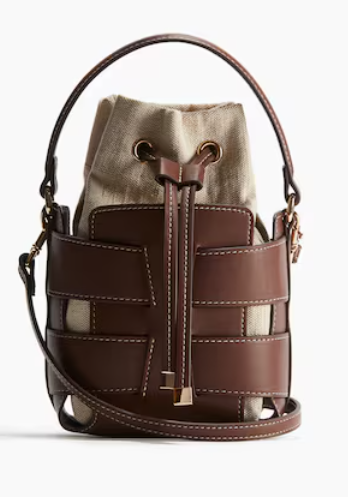
\includegraphics[width=3cm]{8d09e8f949dc460bb77b42ed8fe31187.png}};
  \end{tikzpicture}

  \vspace{3mm}
  {\color{black}\LARGE \textbf{Pape Saliou FALL}}

  \vspace{1mm}
  {\large Ingénieur Data Scientist \& Développeur IA}

  \vspace{3mm}
  {\color{gray}\rule{\linewidth}{0.4pt}} \\
\end{minipage}

% ── Coordonnées
\begin{tabular}{@{}c l}
  \faPhone &
  \begin{tabular}[t]{@{}l@{}}
    {\color{gray}Téléphone} \\ 0753481453
  \end{tabular} \\
  \\
  \faLinkedin &
  \begin{tabular}[t]{@{}l@{}}
    {\color{gray}LinkedIn} \\
    \href{https://linkedin.com/in/pape-saliou-fall-43154a211}{Mon LinkedIn}
  \end{tabular} \\
  \\
  \faMapMarker &
  \begin{tabular}[t]{@{}l@{}}
    {\color{gray}Adresse} \\ 95300 Pontoise \\ 
  \end{tabular} \\
  \\
  \faEnvelope &
  \begin{tabular}[t]{@{}l@{}}
    {\color{gray}Email} \\
    \href{mailto:papesalioufall2@gmail.com}{papesalioufall2@gmail.com}
  \end{tabular} \\
\end{tabular}

\vspace{2mm}
{\color{gray}\rule{\linewidth}{0.4pt}} \\

% ── Langues --------------------------------------------------------
{\color{black}{Langues}}

\vspace{2mm}
\begin{itemize}[leftmargin=*]
\item Français - \textcolor{gray}{C2}
\item Anglais - \textcolor{gray}{B2}\end{itemize}          % ← le placeholder va contenir \begin{itemize}…\end{itemize}

{\color{gray}\rule{\linewidth}{0.4pt}} \\

% ── Compétences ----------------------------------------------------
\vspace{2mm}
{\color{black}{Compétences Clés}}

\vspace{2mm}
\begin{itemize}[leftmargin=*]
\item Python
\item SQL
\item Git
\item TensorFlow
\item PowerBI
\item MachineLearning
\item DeepLearning\end{itemize}              % ← idem, une vraie liste
\vspace{2mm}
{\color{gray}\rule{\linewidth}{0.4pt}} \\

% ── Centres d'intérêt
\vspace{2mm}
{\color{black}{Centres d’intérêt}}

\vspace{2mm}
\begin{itemize}[leftmargin=*]
\item Football
\item Natation
\item Lecture
\item Musique
\end{itemize}     % ← simple itemize ou tabular

\vfill
~

% ────────────────────────────────────────
\switchcolumn
% Colonne droite
% ────────────────────────────────────────
\color{black}

% ── Profil
\textcolor{black}{\Large \textbf{Profil Professionnel}} \\[2pt]
Data Scientist doté d’une solide expertise en analyse de données, machine learning et développement d’applications IA. Habitué à transformer des jeux de données complexes en solutions concrètes, je privilégie la collaboration et la proactivité pour faire avancer les projets. Autonome et curieux, j’aime relever de nouveaux défis techniques et contribuer à des environnements où l’innovation est valorisée. Je recherche désormais une opportunité stimulante pour mettre mon savoir-faire au service de projets ambitieux. \\[8pt]

% ── Expérience
\textcolor{black}{\Large \textbf{Expérience Professionnelle}} \\[2pt]

\colorbox{maincolor}{%
  \begin{minipage}{\linewidth}
    \textbf{Data Scientist \& Développeur IA} \\ Prepaya \\ Jan 2024 – Présent
    \begin{itemize}
      \item Conçu et déployé une plateforme IA full-stack (Python/JavaScript) automatisant les flux de données. \item Implémenté des modèles de prévision sur séries temporelles avec Scikit-learn et TensorFlow, améliorant la précision des prédictions. \item Industrialisé la solution sur Heroku avec PostgreSQL et APIs REST, réduisant les délais de mise en production.
    \end{itemize}
  \end{minipage}}

\vspace{3mm}


\colorbox{maincolor}{%
  \begin{minipage}{\linewidth}
    \textbf{Apprenti Risk Analyst \& Data Scientist} \\ AXA XL (Groupe AXA) \\ Déc 2022 – Déc 2023
    \begin{itemize}
      \item Automatisé la collecte de données financières via Python/VBA, diminuant les tâches manuelles récurrentes. \item Créé des tableaux de bord Power BI pour le suivi de la facturation, offrant une visibilité en temps réel aux équipes finance et management. \item Développé des modèles prédictifs d’occurrence de sinistres, renforçant la prise de décision en gestion des risques.
    \end{itemize}
  \end{minipage}}

\vspace{3mm}


\colorbox{maincolor}{%
  \begin{minipage}{\linewidth}
    \textbf{Apprenti Data Scientist} \\ Prepaya \\ Sept 2021 – Août 2022
    \begin{itemize}
      \item Mis en œuvre des réseaux de neurones NLP (BERT, T5) pour générer automatiquement des formulaires clients. \item Réalisé des analyses de sentiments sur les retours utilisateurs afin de mesurer la satisfaction et guider les améliorations. \item Conçu des scripts de collecte de données textuelles avec BeautifulSoup et Selenium, enrichissant les jeux de données internes.
    \end{itemize}
  \end{minipage}}   % ← blocs \colorbox{maincolor}{\begin{minipage}…}

\vspace{8mm}

% ── Formation
\textcolor{black}{\Large \textbf{Formation}} \\[2pt]

    \begin{tabularx}{\linewidth}{@{}c X@{}}
    \textcolor{sidetext}{\faGraduationCap} &
    \textbf{Master 2 Data Science} \\
    & Sorbonne Université \\
    & \begin{itemize}[leftmargin=*]
  \item Approfondissement des méthodes d’analyse de données, machine learning et deep learning. \item Études de séries temporelles, modèles de structure latente et calcul parallèle sur bases de données volumineuses.
\end{itemize} \\
    & \textit{Sept 2021 – Mars 2022}
    \end{tabularx}
           % ← lignes tabular par diplôme

\end{paracol}
\end{document}

